\chapter{Filtering logical dependencies}
\label{extraction}


\section{Extracting structural dependencies}
\label{sec:sd_extraction}
A dependency is created between two elements that are in a relationship and indicates that an element of the relationship, in some manner, depends on the other element of the relationship \cite{Booch:2004:OAD:975416}, \cite{Cataldo2009SoftwareDW}.

Structural dependencies can be found by analyzing the source code \cite{Sangal:2005:UDM:1094811.1094824}, \cite{CalloArias2011}, \cite{structdep}. A structural dependency between two classes A and B is given by the fact that A statically depends on B, meaning that A cannot be compiled without knowing about B. In object oriented systems, this dependency can be given by many types of relationships between the two classes: A extends B, A implements B, A has attributes of type B, A has methods which have type B in their signature, A uses local variables of type B, A calls methods of B.


 We use an external tool called srcML \cite{srcML} to convert all source code files from the current release into XML files. All the information about classes, methods, calls to other classes are extracted by parsing the XML files and building a dependency data structure \cite{2003:XLC:851042.857028},
\cite{Collard:2011:LTF:2067850.2068011}. We choose the srcML format because it has the same markup for different programming languages and can ease the parsing of source code written in various programming languages such as Java, C++, and C\#.


\section{Extracting co-changing pairs}
\label{sec:copairs_extraction}

\textit{Logical dependencies} (a.k.a logical coupling) can be found by software history analysis and can reveal relationships that are not always present in the source code (structural dependencies).  

TBA

\section{Tool for measuring software dependencies}
\label{sec:tool}

To establish structural and logical dependencies, we developed a tool that takes as input the source code repository URL of a given system and extracts from it the software dependencies \cite{DepSACI}. 
From a workflow point of view, we can identify 3 major types of activities that the tool does: downloads the required data from the git repository, extracts from the source code the structural dependencies and, extracts and filters the co-changing pairs from the repository's commit history. Figure \ref{fig:figworkflow} represents the activities mentioned above. Each block represents a different activity. 

\begin{figure}[H]
\centering
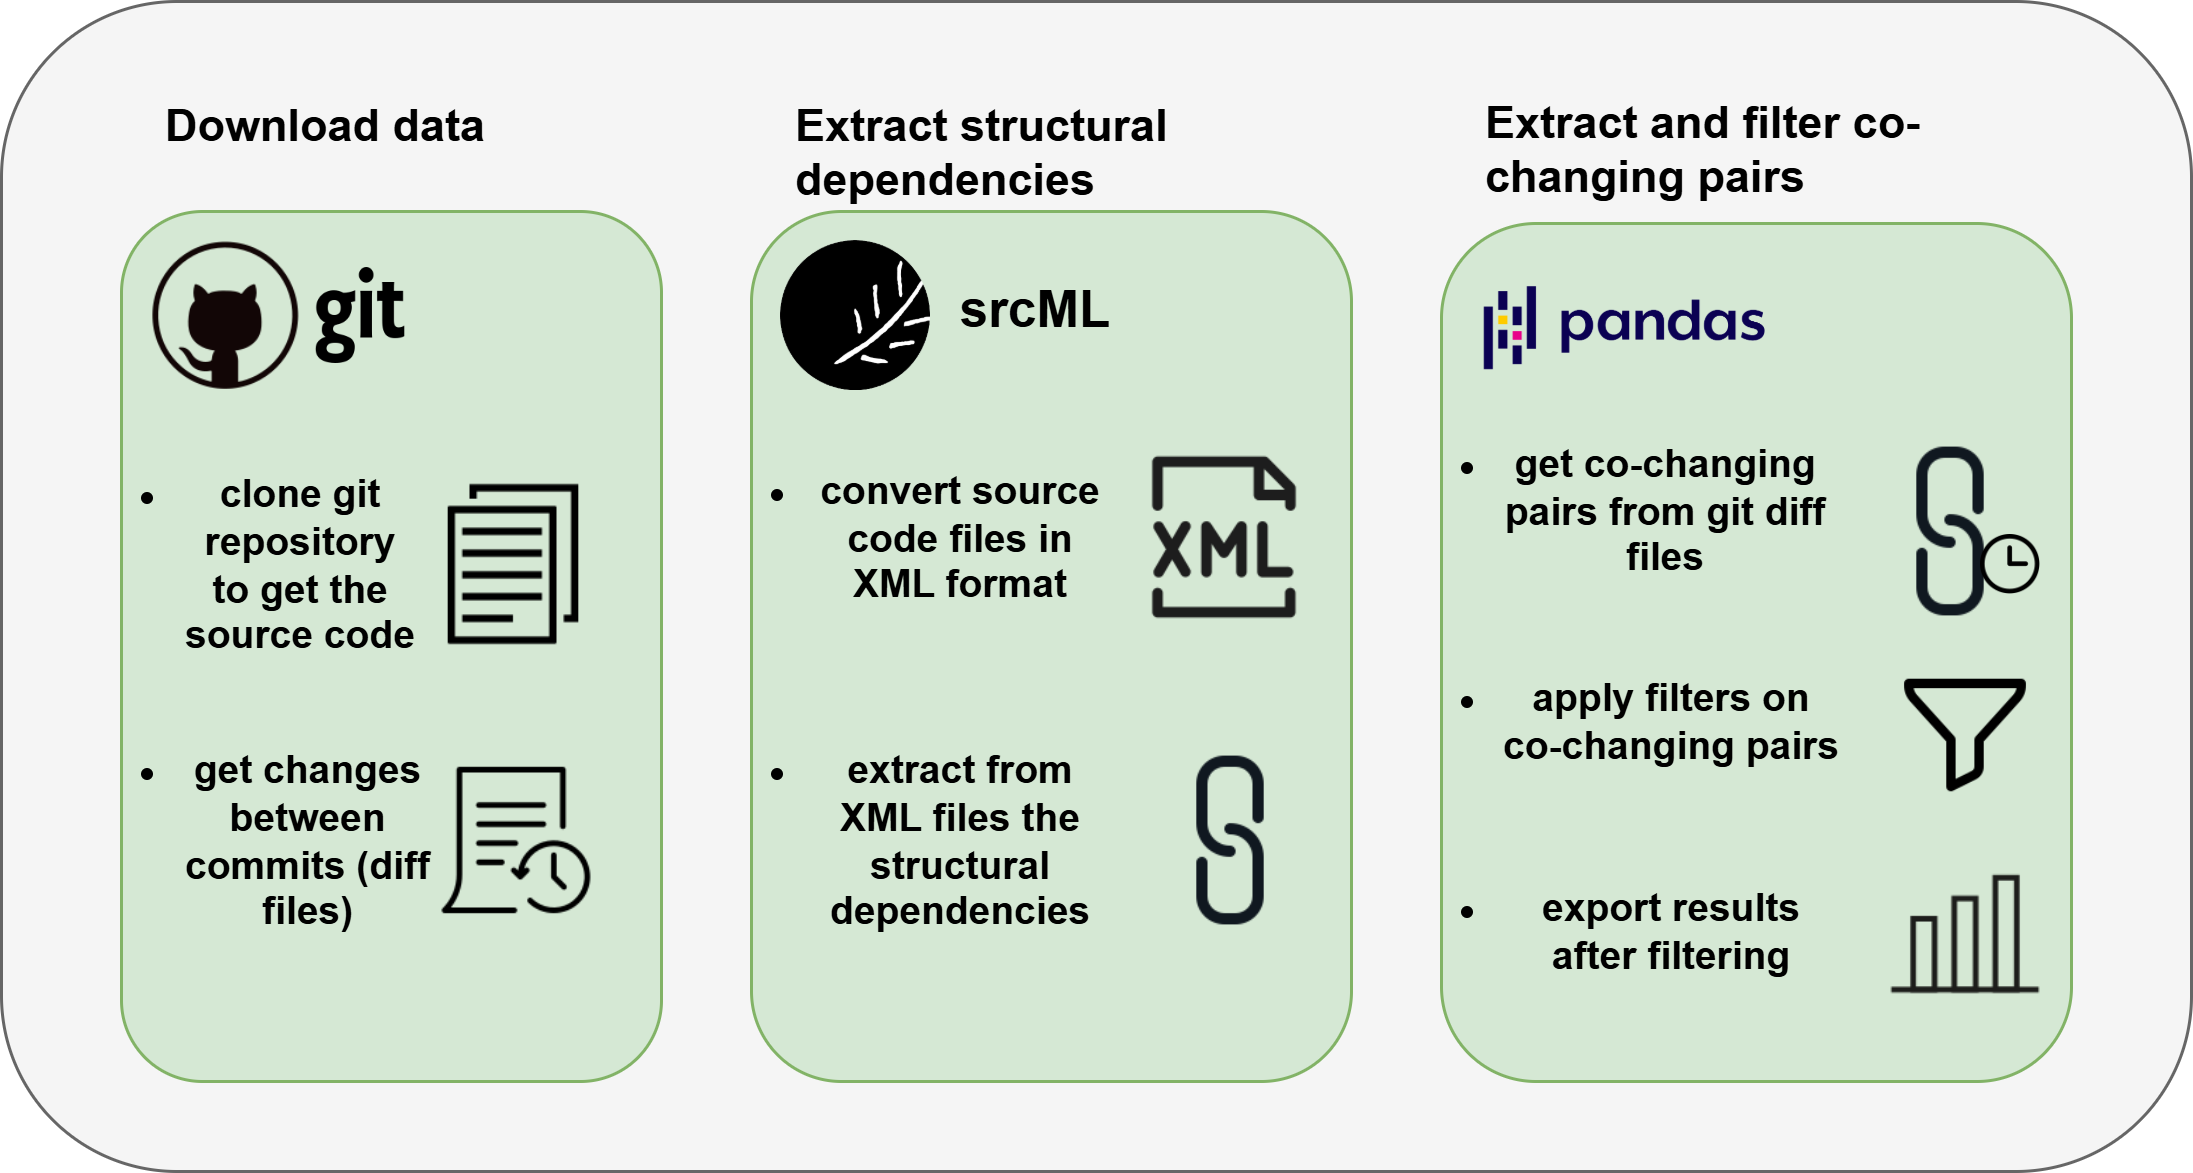
\includegraphics[width=\textwidth]{tool_workflow.png}
\caption{Tool workflow and major activities.}
\label{fig:figworkflow}
\end{figure}


\textbf{Download git data.}

The source code repository provides us all the needed information to extract both types of dependencies. It holds the code of the system but also the change history of the system. We use the source code for structural dependencies extraction and the change history for co-changing pairs extraction.
To get the source code files and the change history, we first need to know the repository URL from GitHub (GitHub is a Git repository cloud-based hosting service). With the GitHub URL and a series of Git commands, the tool can download all the necessary data for dependencies extraction.

As we can see in figure \ref{fig:figgitdata}, the \textit{"clone"} command will download a Git repository to your local computer, including the source code files. The \textit{"diff"} command will get the differences between two existing commits in the Git repository. 
The tool gets the Git repository and the source code files by executing the "clone" command. Afterward, it gets all the existing commits within the Git repository. The commits are ordered by date, beginning with the oldest one and ending with the most recent one. The tool executes the "diff" command between each commit and its parent (the previous commit). The "diff" command generates a text file that contains the differences between the two commits: code differences, the number of files changed and changed file names.


\begin{figure}[H]
\centering
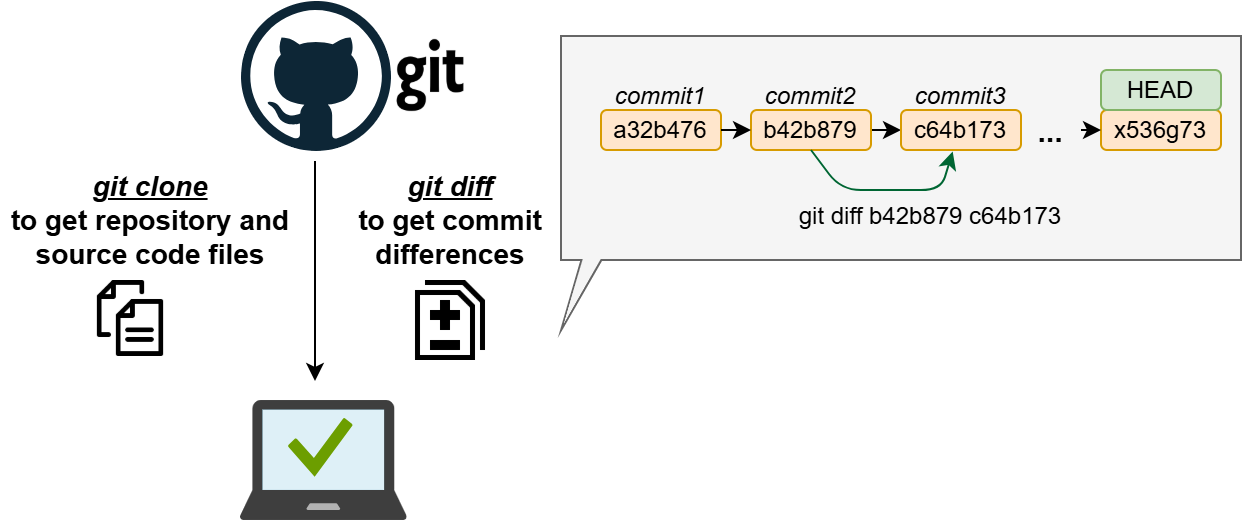
\includegraphics[width=\textwidth]{gitdata.png}
\caption{Commands used to download the required data from GitHub.}
\label{fig:figgitdata}
\end{figure}

\textbf{Extract structural dependencies.}

To extract the structural dependencies from the source code files the tool converts each source code file into srcML format using an open-source tool called srcML. The srcML format is an XML representation for source code. Each markup tag identifies elements of the abstract syntax for the language \cite{srcML}. 
After conversion, the tool parses each file and identifies all the defined entities (class, interface, enum, struct) within the file. It also identifies all the entities that are used by the entities defined.  The connection between both types of entities mentioned above constitutes a structural dependency.

\textbf{Extract and filter co-changing pairs.}

The process of extracting and filtering the co-changing pairs is represented in figure \ref{fig:figfiltering}.
For co-changing pairs extraction, the tool parses each generated diff file.
For each file, the tool gets the number of changed files and the name of the files. 
After structural dependencies extraction, the tool knows all the software entities contained in a file. Two entities from two changed files form a co-changing pair. After all the co-changing pairs of one diff file are extracted, the tool moves to the next diff file and extracts the set of co-changing pairs.

As will be presented in more details in sections \ref{sec:filtercommit}, \ref{sec:filterocc}, and \ref{sec:filterstrength}, not every co-changing pair extracted is a logical dependency. For a co-changing pair to be labeled as a logical dependency, it has to meet some criteria. Each criterion constitutes a filter that a co-changing pair has to pass in order to be called logical dependency.
The filters are implemented in the tool and can be combined. The input for each filter is the set of co-changing pairs extracted, and the output is the remaining co-changing pairs that respect the filter criterion.


\begin{figure}[H]
\centering
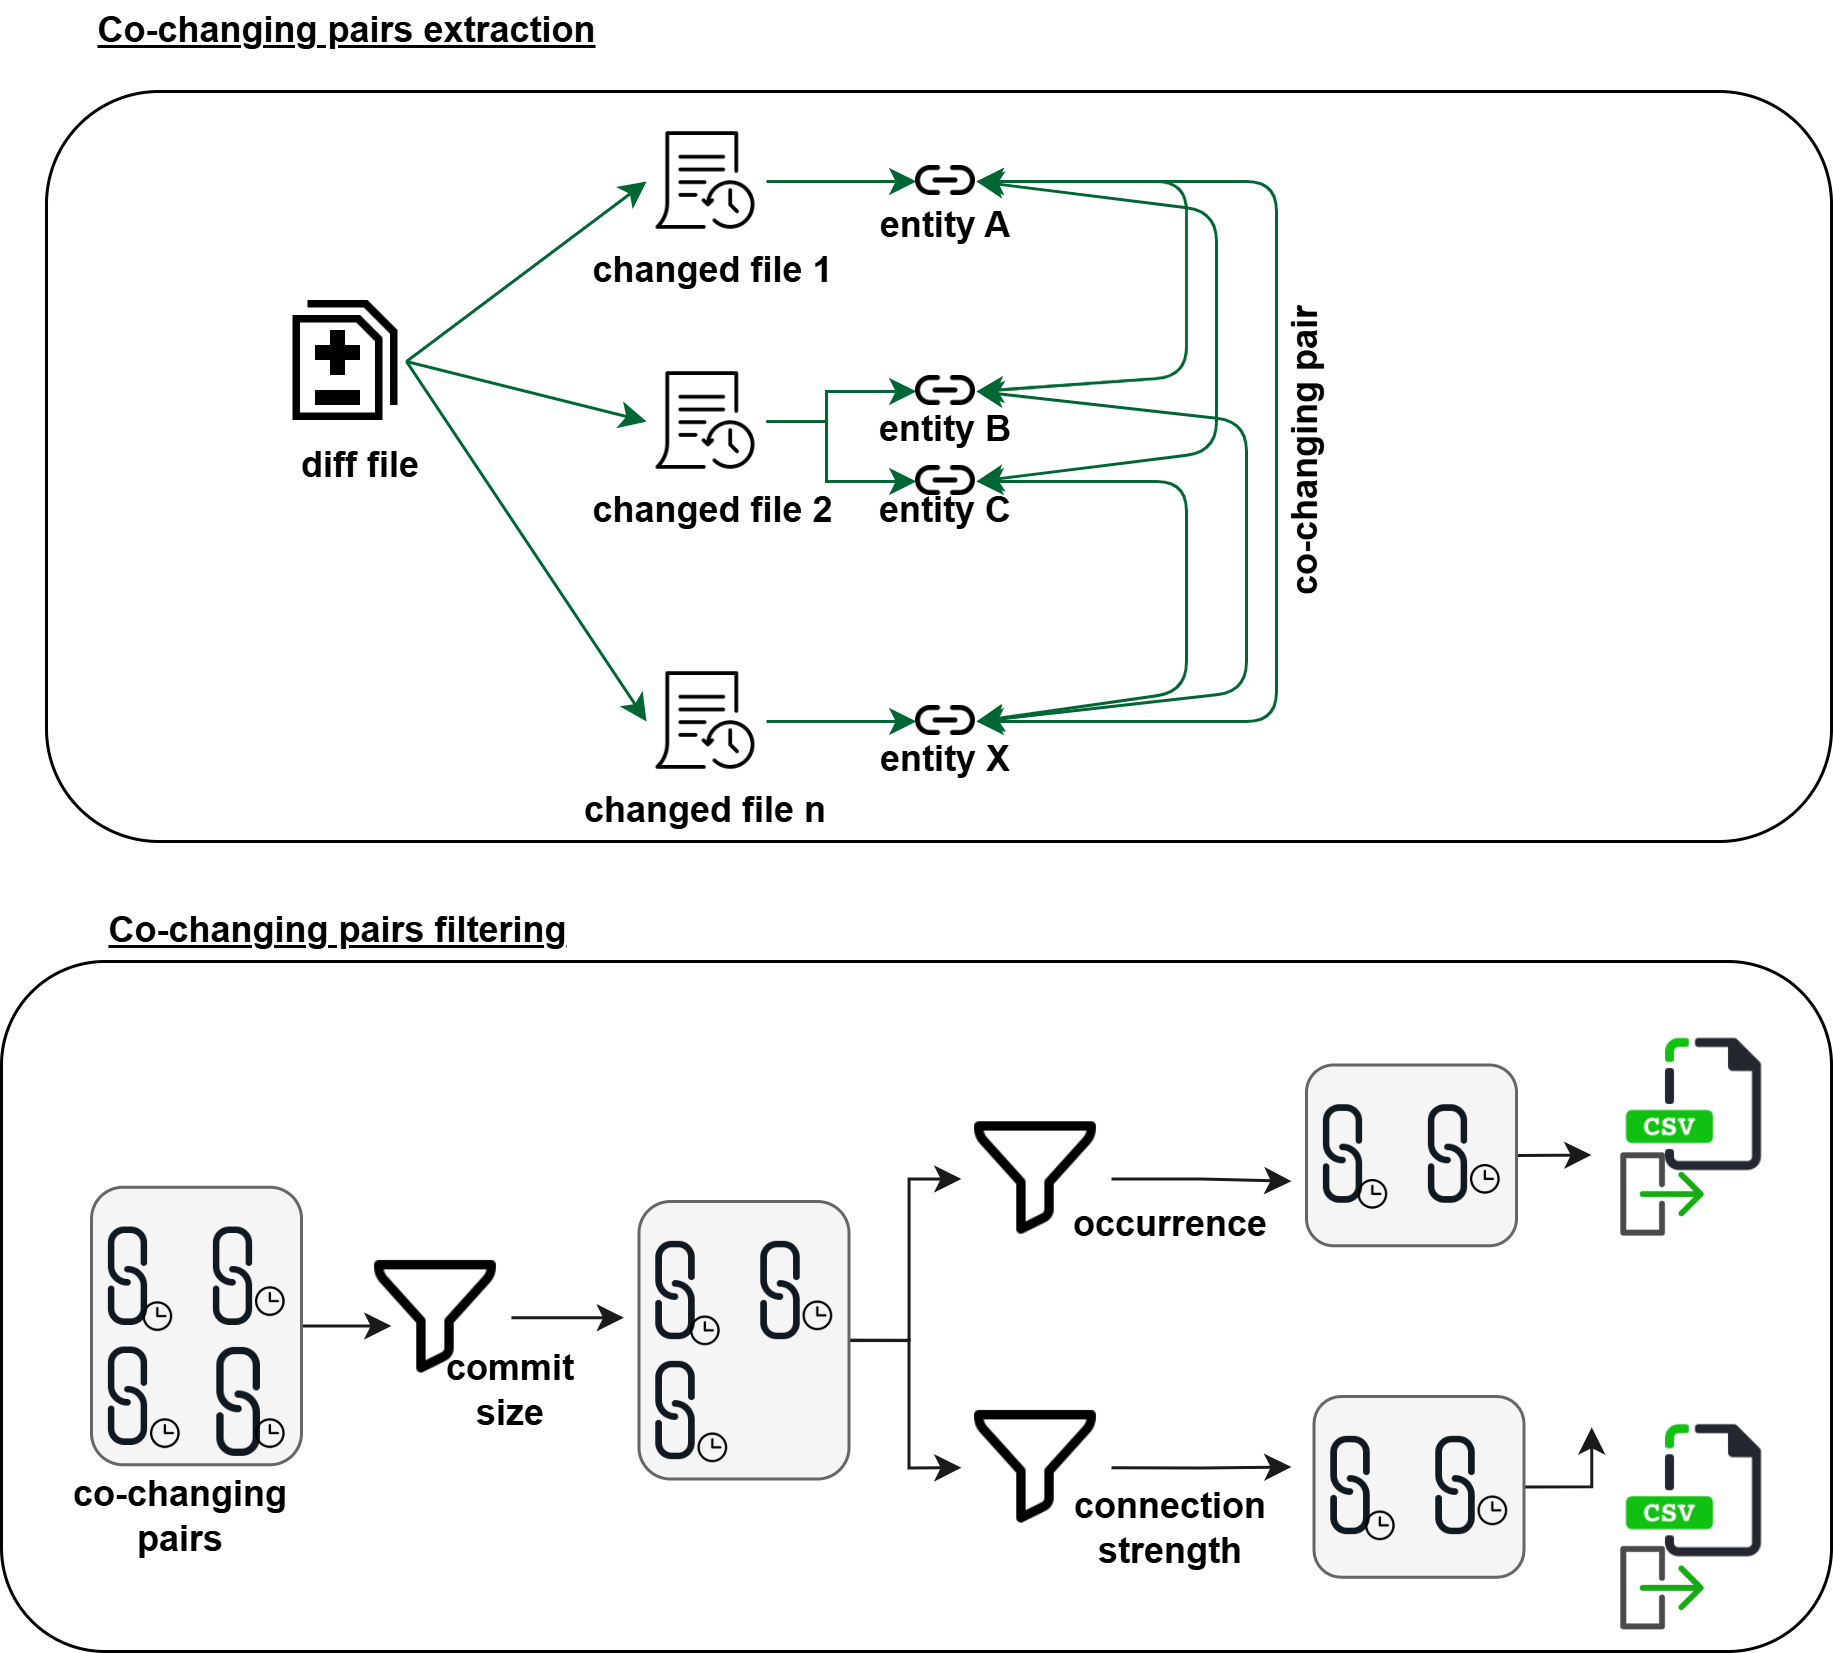
\includegraphics[width=\textwidth]{pairs_filtering.png}
\caption{Co-changing pairs extraction and filtering.}
\label{fig:figfiltering}
\end{figure}


\section{Data set used}
\label{sec:dataset}
We have analyzed a set of open-source projects found on GitHub\footnote{http://github.com/} \cite{Kalliamvakou2016} in order to extract the structural and logical dependencies between classes. Table \ref{table:1} enumerates all the systems studied. The 1st column assigns the projects IDs; 2nd column shows the project name; 3rd column shows the number of entities(classes and interfaces) extracted; 4th column shows the number of most recent commits analyzed from the active branch of each project and the 5th shows the language in which the project was developed.


\begin{table}[!h]
\renewcommand{\arraystretch}{1}
\caption{Summary of open source projects studied.}
\label{table:1}
\centering
\scalebox{0.9}{
\begin{tabular}{|c|c|c|c|c|c|}
\hline
   ID  & Project    & Nr. of & Nr. of& Type\\
     &     & entites & commits & \\
\hline
1	&	bluecove	&	2685	&	894	&	java	\\
2	&	aima-java	&	5232	&	1006	&	java	\\
3	&	powermock	&	2801	&	949	&	java	\\
4	&	restfb	&	3350	&	1391	&	java	\\
5	&	rxjava	&	21097	&	4398	&	java	\\
6	&	metro-jax-ws	&	6482	&	2927	&	java	\\
7	&	mockito	&	5189	&	3330	&	java	\\
8	&	grizzly	&	10687	&	3113	&	java	\\
9	&	shipkit	&	639	&	1563	&	java	\\
10	&	OpenClinica	&	9655	&	3276	&	java	\\
11	&	robolectric	&	8922	&	5912	&	java	\\
12	&	aeron	&	4159	&	5977	&	java	\\
13	&	antlr4	&	4747	&	4431	&	java	\\
14	&	mcidasv	&	3272	&	4136	&	java	\\
15	&	ShareX	&	4289	&	5485	&	csharp	\\
16	&	aspnetboilerplate	&	9712	&	4323	&	csharp	\\
17	&	orleans	&	16963	&	3995	&	csharp	\\
18	&	cli	&	2063	&	4488	&	csharp	\\
19	&	cake	&	12260	&	2518	&	csharp	\\
20	&	Avalonia	&	16732	&	5264	&	csharp	\\
21	&	EntityFrameworkCore	&	50179	&	5210	&	csharp	\\
22	&	jellyfin	&	8764	&	5433	&	csharp	\\
23	&	PowerShell	&	2405	&	3250	&	csharp	\\
24	&	WeiXinMPSDK	&	7075	&	5729	&	csharp	\\
25	&	ArchiSteamFarm	&	702	&	2497	&	csharp	\\
26	&	VisualStudio	&	4869	&	5039	&	csharp	\\
27	&	CppSharp	&	17060	&	4522	&	csharp	\\

\hline
\end{tabular}
}
\end{table}

\section{Overview in types of filters used}

\subsection{Filtering based on the size of commit transactions}
\label{sec:filtercommit}

As presented in section \ref{sec:copairs_extraction}, according to surveys,  co-changing pairs are not used because of their size. One system can have millions of co-changing pairs.
With this filtering type, we not only want to decrease the total size of the extracted co-changing pairs. But also to be one step closer to the identification of the logical dependencies among the co-changing pairs.
In this step, we want to filter the co-changing pairs extracted after commit size (cs). This means that the co-changing pairs are extracted only from commits that involve fewer files than an established threshold number. 

Different works have chosen fixed threshold values for the maximum number of files accepted in a commit. Cappiluppi and Ajienka, in their works \cite{DBLP:journals/jss/AjienkaC17}, \cite{DBLP:journals/ese/AjienkaCC18} only take into consideration commits with less then 10 source code files changed in building the logical dependencies.

The research of Beck et al \cite{Beck:2011:CMC:2025113.2025162} only takes in consideration transactions with up to 25 files. The research \cite{Oliva:2011:ISL:2067853.2068086} provided also a quantitative analysis of the number of files per revision; Based on the analysis of 40,518 revisions, the mean value obtained for the number of files in a revision is 6 files. However, standard deviation value shows that the dispersion is high. 

We analyzed the overall transaction size trend for 27 open-source csharp and java systems with a total of 74 332 commits. The results are presented in Figure \ref{fig:fig_cs} and in table \ref{table:cs_values}, based on them we can say that 90\% of the total commit transactions made are with less than 10 source code files changed. This percent allows us to say that setting a threshold of 10 files for the maximum size of the commit transactions will not affect so much the total number of commit transactions from the systems since it will still remain 90\% of the commit transactions from where we can extract co-changing pairs \cite{DepSACI}.


\begin{figure}[!h]
\centering
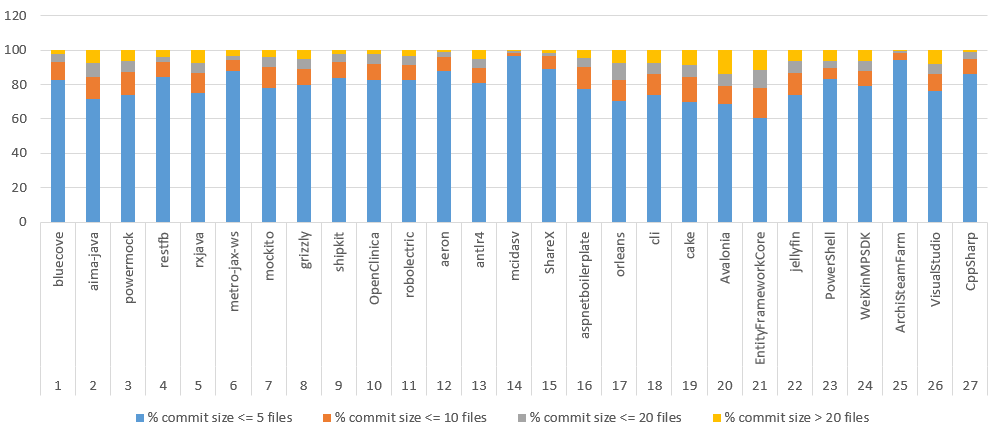
\includegraphics[width=\textwidth]{commit_distribution.png}
\caption{Commit transaction size(cs) trend in percentages.}
\label{fig:fig_cs}
\centering
\end{figure}


\begin{figure}[!h]
\centering
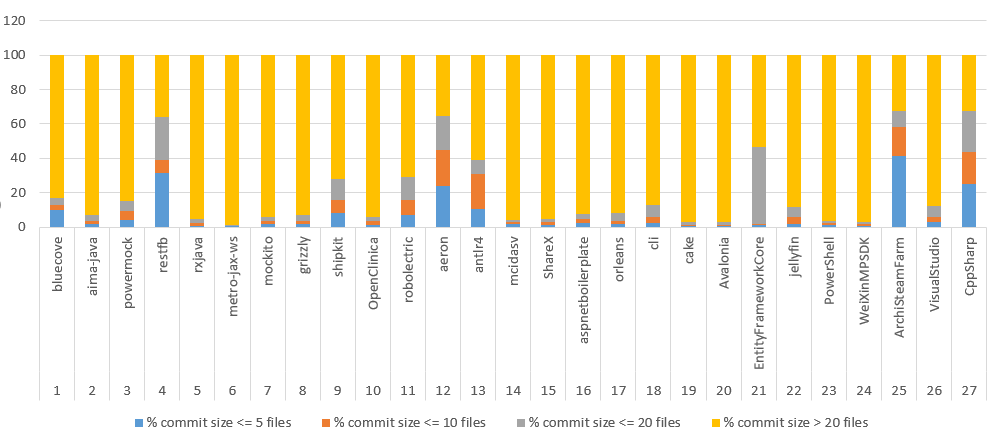
\includegraphics[width=\textwidth]{ld_distribution.png}
\caption{Percentages of LD extracted from each commit transaction size(cs) group.}
\label{fig:fig_ld_cs}
\centering
\end{figure}

As we can see in Figure \ref{fig:fig_ld_cs} even though only 5\% of the commit transactions have more than 20 files changed ($20<cs<inf$) they generate in average 80\% of the total amount of co-changing pairs extracted from the systems.
The high number of co-changing pairs extracted from such a small number of commit transactions is caused by the number of files involved in those commit transactions. 

One single commit transaction can lead to a large amount of co-changing pairs. For example in RxJava we have commit transactions with 1030 source code files, this means that those commits can generate 
$\Comb{n}{k}=\frac{n!}{k!(n-k)!} = \frac{1030!}{2!(1028)!} = 529 935$ logical dependencies. By setting a threshold on the commit transaction size we can avoid the introduction of those co-changing pairs into the system.



So filtering 10\% of the total amount of commit transactions can lead to a significant decrease of the amount of co-changing pairs and that is why we choose the value of 10 files as our fixed threshold for the maximum size of a commit transaction \cite{DepSACI}.



\begin{table}[!h]
\renewcommand{\arraystretch}{1}
\caption{Commit transaction size(cs) trend and average per system.}
\label{table:cs_values}
\centering
\scalebox{0.9}{
\begin{tabular}{|c|c|c|c|c|c|c|}
\hline
Nr.	  & Project    &	$cs\leq 5$	&	$cs\leq 10$	&	$cs\leq 20$	&	$cs<\infty$ & Avg	\\ 
\hline
1	&	bluecove	&	738	&	97	&	37	&	22	&	4.9	\\
2	&	aima-java	&	733	&	134	&	74	&	65	&	7.24	\\
3	&	powermock	&	685	&	128	&	66	&	70	&	9.61	\\
4	&	restfb	&	1160	&	127	&	44	&	60	&	9.9	\\
5	&	rxjava	&	3395	&	447	&	253	&	303	&	8.46	\\
6	&	metro-jax-ws	&	2583	&	198	&	78	&	68	&	4.33	\\
7	&	mockito	&	2522	&	433	&	222	&	153	&	6.33	\\
8	&	grizzly	&	2487	&	302	&	180	&	144	&	5.28	\\
9	&	shipkit	&	1311	&	151	&	64	&	37	&	4.26	\\
10	&	OpenClinica	&	2837	&	250	&	119	&	70	&	3.31	\\
11	&	robolectric	&	4827	&	503	&	264	&	318	&	7.43	\\
12	&	aeron	&	4844	&	684	&	300	&	149	&	4.6	\\
13	&	antlr4	&	3426	&	437	&	304	&	264	&	8.5	\\
14	&	mcidasv	&	3996	&	81	&	35	&	24	&	2.47	\\
15	&	ShareX	&	4731	&	529	&	145	&	80	&	4.69	\\
16	&	aspnetboilerplate	&	3208	&	569	&	321	&	225	&	6.61	\\
17	&	orleans	&	2780	&	518	&	369	&	328	&	8.95	\\
18	&	cli	&	3377	&	551	&	308	&	252	&	6.43	\\
19	&	cake	&	1785	&	359	&	174	&	200	&	9.89	\\
20	&	Avalonia	&	3806	&	641	&	371	&	446	&	8.43	\\
21	&	EntityFrameworkCore	&	2866	&	878	&	644	&	822	&	15.38	\\
22	&	jellyfin	&	4007	&	662	&	419	&	345	&	6.25	\\
23	&	PowerShell	&	2702	&	224	&	133	&	191	&	7.33	\\
24	&	WeiXinMPSDK	&	4604	&	526	&	296	&	303	&	9.01	\\
25	&	ArchiSteamFarm	&	2357	&	92	&	28	&	20	&	2.24	\\
26	&	VisualStudio	&	3902	&	521	&	295	&	321	&	6.71	\\
27	&	CppSharp	&	3870	&	390	&	203	&	59	&	3.28	\\
\hline
\end{tabular}
}
\end{table}





\subsection{Filtering based on number of occurrences}
\label{sec:filterocc}

In the previous section, we filtered the co-changing pairs based on the commit size. Even though the number of extracted co-changing pairs was reduced, this type of filtering will not guarantee that the remaining co-changing pairs can pass as logical dependencies. 
One occurrence of a co-change pair can be a valid logical dependency, but can also be a coincidence. 

Taking into consideration only co-changing pairs with multiple occurrences as valid dependencies can lead to more accurate results. But, if the project studied has a relatively small amount of commits, the probability to find multiple updates of the same classes at the same time is less likely to happen, so filtering after the number of occurrences can lead to filtering all the co-changes extracted.

We have performed a series of analyses on the test systems, incrementing the threshold value occurrence (occ) from 1 to 4. The co-changing pairs are extracted only for commits with the commit transaction size less or equal to 10. For each threshold mentioned above, the extracted co-changing pairs are filtered again by the occurrence threshold established. All the co-changing pairs that do not exceed the minimum number of occurrences are discarded.

The results of the analysis are presented in Table \ref{table:sd_percentages} as percentages of co-changing pairs that are also structural dependencies and Table \ref{table:ld_ratio} as ratio of the number of co-changing pairs to the number of structural dependencies (SD).


\begin{table}[!h]
\renewcommand{\arraystretch}{1}
\caption{Percentage of co-changing pairs that are also structural dependencies.}
\label{table:sd_percentages}
\centering
\scalebox{0.9}{
\begin{tabular}{|c|c|c|c|c|}
\hline
    ID  & $occ\geq 1$ & $occ\geq 2$ & $occ\geq 3$ & $occ\geq 4$  \\
\hline
1	&	7,13	&	7,77	&	7,99	&	19,71	\\
2	&	19,54	&	25,76	&	29,55	&	32,16	\\
3	&	6,66	&	8,58	&	11,82	&	14,87	\\
4	&	1,16	&	1,17	&	0,91	&	0,80	\\
5	&	3,99	&	3,96	&	7,75	&	7,49	\\
6	&	13,92	&	20,16	&	22,91	&	22,77	\\
7	&	8,38	&	9,28	&	14,93	&	14,58	\\
8	&	6,70	&	9,73	&	14,20	&	15,60	\\
9	&	16,98	&	23,34	&	29,22	&	32,89	\\
10	&	8,94	&	9,15	&	11,05	&	10,59	\\
11	&	4,99	&	6,92	&	8,88	&	11,08	\\
12	&	13,19	&	17,15	&	18,60	&	19,57	\\
13	&	2,43	&	5,59	&	8,33	&	8,21	\\
14	&	13,27	&	18,88	&	19,02	&	19,28	\\
15	&	12,90	&	21,95	&	25,51	&	27,01	\\
16	&	13,33	&	17,34	&	18,53	&	16,24	\\
17	&	6,09	&	6,18	&	6,41	&	6,44	\\
18	&	9,73	&	10,60	&	14,27	&	18,80	\\
19	&	10,26	&	13,54	&	13,64	&	12,60	\\
20	&	12,83	&	18,36	&	21,00	&	25,72	\\
21	&	2,86	&	4,65	&	5,70	&	4,98	\\
22	&	5,20	&	6,56	&	8,18	&	8,90	\\
23	&	8,23	&	13,64	&	17,04	&	17,65	\\
24	&	6,77	&	10,89	&	14,47	&	16,05	\\
25	&	9,85	&	10,15	&	11,65	&	11,33	\\
26	&	8,65	&	10,79	&	12,78	&	14,34	\\
27	&	7,04	&	8,78	&	9,87	&	10,08	\\
\hline
Avg	&	8,93	&	11,88	&	14,23	&	15,55	\\
\hline
\end{tabular}
}
\end{table}


\begin{table}[!h]
\renewcommand{\arraystretch}{1}
\caption{Ratio of number of co-changing pairs to number of structural dependencies. }
\label{table:ld_ratio}
\centering
\scalebox{0.9}{
\begin{tabular}{|c|c|c|c|c|}
\hline
    ID  & $occ\geq 1$ & $occ\geq 2$ & $occ\geq 3$ & $occ\geq 4$  \\
\hline
1	&	4,13	&	1,94	&	1,23	&	0,26	\\
2	&	0,81	&	0,33	&	0,16	&	0,10	\\
3	&	5,12	&	1,93	&	0,78	&	0,38	\\
4	&	53,36	&	42,00	&	38,31	&	36,30	\\
5	&	4,27	&	2,90	&	0,88	&	0,72	\\
6	&	1,07	&	0,46	&	0,30	&	0,23	\\
7	&	4,09	&	2,38	&	0,99	&	0,73	\\
8	&	4,06	&	1,57	&	0,76	&	0,49	\\
9	&	3,64	&	2,03	&	1,14	&	0,77	\\
10	&	1,41	&	1,01	&	0,47	&	0,34	\\
11	&	7,91	&	4,47	&	2,93	&	2,03	\\
12	&	3,92	&	2,15	&	1,47	&	1,07	\\
13	&	10,15	&	3,18	&	1,22	&	1,03	\\
14	&	3,07	&	1,53	&	1,16	&	0,97	\\
15	&	2,34	&	0,84	&	0,48	&	0,33	\\
16	&	1,21	&	0,47	&	0,26	&	0,19	\\
17	&	2,99	&	1,83	&	1,11	&	0,84	\\
18	&	2,26	&	1,37	&	0,67	&	0,40	\\
19	&	2,32	&	1,38	&	0,76	&	0,67	\\
20	&	1,24	&	0,58	&	0,35	&	0,18	\\
21	&	5,33	&	2,12	&	1,27	&	1,05	\\
22	&	3,38	&	1,88	&	0,99	&	0,74	\\
23	&	3,62	&	1,22	&	0,76	&	0,37	\\
24	&	2,57	&	1,22	&	0,67	&	0,46	\\
25	&	7,47	&	5,36	&	4,16	&	3,73	\\
26	&	4,03	&	2,16	&	1,50	&	1,15	\\
27	&	7,46	&	4,26	&	2,99	&	2,43	\\
\hline
Avg	&	5,67	&	3,43	&	2,51	&	2,15	\\
\hline
\end{tabular}
}
\end{table}

Based on Table \ref{table:sd_percentages} we can say that only a small percentage of the extracted co-changing pairs are also structural dependencies. This is consistent with the findings of related works \cite{DBLP:journals/jss/AjienkaC17}, \cite{DBLP:journals/ese/AjienkaCC18}. 
The percentage of co-changing pairs that are also structural dependencies increases with the minimum number of occurrences because the number of co-changing pairs from the systems decreases with the minimum number of occurrences. 
We calculate the overlapping between co-changing pairs and structural dependencies not only because we want to get an idea of how many structural dependencies are reflected in the versioning system through co-changing pairs, but also because we want to eliminate co-changing pairs that are structural dependencies since they don't bring any new information about the system.

We stopped the minimum occurrences threshold to 4 because we observed that for systems with ID 2, 6, 10, and 16 from Table \ref{table:ld_ratio} the ratio number is lower than 1, which means that the number of structural dependencies is higher than the number of co-changing pairs. On the other hand, for systems with ID 4, 11, 25, 27, the threshold of 4 for a minimum number of occurrences does not change the discrepancy between the number of co-changing pairs and structural dependencies.

If we try to go higher with the occurrences threshold, we will risk filtering all the existing co-changing pairs for some systems.
So, filtering with a threshold of 4 for the minimum number of occurrences will indeed filter the logical dependencies, but for some of the systems, the remaining number of co-changing pairs will still be significantly higher compared to the number of structural dependencies.




\subsection{Filtering based on connection strength}
\label{sec:filterstrength}

In section \ref{sec:filtercommit} we filtered the co-changing pairs extracted from the versioning system history based on the commit size. Based on the results obtained, we decided to filter out all co-changing pairs extracted from commits with more than 10 files changed. 

In section \ref{sec:filterocc}, we added a new filtering rule based on the occurrence of a co-changing pair. The new filter is applied to the co-changing pairs resulted after commit size filtering. In this case, the filtering method proved insufficient due to the size diversity of the systems. One important conclusion drawn from the occurrence number filtering is that setting a hard threshold for a filter is not always a good idea. One threshold value can be too much for a small-sized system and too little for a medium-sized system. 

To avoid the above problem, we decided to introduce another filter complementary to the commit size filter described in section \ref{sec:filtercommit}.
This filter focuses on the connection strength of a co-changing pair. In this section, we will filter out all the co-changing pairs that are not strongly connected.

To determine the connection strength of a pair, we first need to calculate the connection factors for both entities that form a co-changing pair.
Assuming that we have a co-changing pair formed by entities A and B, the connection factor of entity A with entity B is the percentage from the total commits involving A that contains entity B. The connection factor of entity B with entity A is the percentage from the total commits involving B that contain also entity A.

\begin{equation}
 connection\ factor\ for\ A = \frac{100 * commits\ involving\ A\ and\ B}{total\ nr\ of\ commits\ involving\ A}
\end{equation}

\begin{equation}
 connection\ factor\ for\ B = \frac{100 * commits\ involving\ A\ and\ B}{total\ nr\ of\ commits\ involving\ B}
\end{equation}

As a practical example, if the pair formed by A and B update together 7 times and the total number of commits involving A is 20 and involving B is 7. The factor for A is 35 and for B is 100. The factor of 100 is the maximum factor that you can have and means that in all the commits involving B, also A is present.

Due to the fact that the factors obtained can vary from 0 to 100, for this filter, we begin with a threshold value of 10 and increment it by 10 until we reach 100. 

The co-changing pairs are filtered out based on two scenarios:
\begin{itemize}
	\item factor A and factor B $\geq threshold \%$ 
	\item factor A or factor B $\geq threshold \%$ 
\end{itemize}

\begin{table}[!h]
\renewcommand{\arraystretch}{1}
\caption{Ratio of number of filtered co-changing pairs to number of SD, when factor A and factor B $\geq threshold \%$ }
\label{tab:commitstrengthAND}
\centering
\scalebox{0.8}{
\begin{tabular}{|c|cccccccccc|c|}
\hline
Project &	$\geq10\%$	&	$\geq20\%$		&	$\geq30\%$		&	$\geq40\%$		&	$\geq50\%$		&	$\geq60\%$		&	$\geq70\%$		&	$\geq80\%$		&	$\geq90\%$		&	$\geq100\%$	 \\
\hline
bluecove	&	1.326	&	0.658	&	0.433	&	0.401	&	0.244	&	0.199	&	0.195	&	0.022	&	0.011	&	0.011	\\
aima-java	&	0.266	&	0.137	&	0.070	&	0.044	&	0.036	&	0.019	&	0.005	&	0.004	&	0.003	&	0.003	\\
powermock	&	0.505	&	0.243	&	0.147	&	0.086	&	0.061	&	0.031	&	0.031	&	0.031	&	0.031	&	0.031	\\
restfb	&	0.822	&	0.163	&	0.045	&	0.017	&	0.011	&	0.002	&	0.001	&	0.001	&	0.001	&	0.001	\\
rxjava	&	0.234	&	0.119	&	0.054	&	0.037	&	0.034	&	0.018	&	0.013	&	0.011	&	0.007	&	0.007	\\
metro-jax-ws	&	0.227	&	0.155	&	0.101	&	0.077	&	0.070	&	0.036	&	0.018	&	0.017	&	0.016	&	0.016	\\
mockito	&	1.590	&	0.804	&	0.357	&	0.288	&	0.215	&	0.088	&	0.052	&	0.036	&	0.032	&	0.032	\\
grizzly	&	2.073	&	0.293	&	0.170	&	0.111	&	0.093	&	0.050	&	0.039	&	0.034	&	0.021	&	0.007	\\
shipkit	&	1.495	&	0.479	&	0.271	&	0.142	&	0.108	&	0.059	&	0.047	&	0.011	&	0.008	&	0.008	\\
OpenClinica	&	0.253	&	0.135	&	0.093	&	0.078	&	0.062	&	0.042	&	0.024	&	0.019	&	0.019	&	0.017	\\
robolectric	&	0.114	&	0.086	&	0.064	&	0.037	&	0.027	&	0.025	&	0.001	&	0.000	&	0.000	&	0.000	\\
aeron	&	0.277	&	0.136	&	0.085	&	0.069	&	0.053	&	0.045	&	0.039	&	0.015	&	0.007	&	0.004	\\
antlr4	&	11.363	&	0.721	&	0.031	&	0.010	&	0.007	&	0.004	&	0.000	&	0.000	&	0.000	&	0.000	\\
mcidasv	&	3.225	&	0.805	&	0.660	&	0.533	&	0.493	&	0.454	&	0.386	&	0.356	&	0.005	&	0.005	\\
ShareX	&	6.097	&	0.725	&	0.663	&	0.564	&	0.500	&	0.242	&	0.176	&	0.170	&	0.001	&	0.001	\\
aspnetboilerplate	&	1.302	&	0.333	&	0.219	&	0.146	&	0.094	&	0.045	&	0.014	&	0.008	&	0.007	&	0.007	\\
orleans	&	0.816	&	0.640	&	0.551	&	0.503	&	0.496	&	0.196	&	0.159	&	0.152	&	0.142	&	0.142	\\
cli	&	1.676	&	0.233	&	0.159	&	0.118	&	0.102	&	0.062	&	0.058	&	0.029	&	0.026	&	0.026	\\
cake	&	2.335	&	0.753	&	0.614	&	0.337	&	0.075	&	0.021	&	0.007	&	0.004	&	0.004	&	0.004	\\
Avalonia	&	0.846	&	0.117	&	0.098	&	0.018	&	0.013	&	0.002	&	0.001	&	0.001	&	0.001	&	0.001	\\
EntityFrameworkCore	&	3.377	&	1.691	&	1.608	&	1.584	&	1.576	&	1.310	&	0.001	&	0.001	&	0.001	&	0.001	\\
jellyfin	&	0.132	&	0.006	&	0.003	&	0.002	&	0.002	&	0.000	&	0.000	&	0.000	&	0.000	&	0.000	\\
PowerShell	&	1.732	&	1.299	&	0.158	&	0.053	&	0.007	&	0.001	&	0.000	&	0.000	&	0.000	&	0.000	\\
WeiXinMPSDK	&	3.295	&	0.334	&	0.188	&	0.061	&	0.017	&	0.006	&	0.003	&	0.001	&	0.000	&	0.000	\\
ArchiSteamFarm	&	0.897	&	0.479	&	0.429	&	0.423	&	0.412	&	0.403	&	0.339	&	0.009	&	0.001	&	0.000	\\
VisualStudio	&	1.281	&	0.090	&	0.053	&	0.028	&	0.020	&	0.013	&	0.006	&	0.001	&	0.001	&	0.001	\\
CppSharp	&	99.528	&	1.020	&	0.992	&	0.980	&	0.972	&	0.927	&	0.078	&	0.075	&	0.073	&	0.072	\\

\hline
\end{tabular}
}
\end{table}


\begin{table}[!h]
\renewcommand{\arraystretch}{1}
\caption{Ratio of number of filtered co-changing pairs to number of SD,
 when factor A or factor B $\geq threshold \%$ }
\label{tab:commitstrengthOR}
\centering
\scalebox{0.8}{
\begin{tabular}{|c|cccccccccc|c|}
\hline
Project &	$\geq10\%$	&	$\geq20\%$		&	$\geq30\%$		&	$\geq40\%$		&	$\geq50\%$		&	$\geq60\%$		&	$\geq70\%$		&	$\geq80\%$		&	$\geq90\%$		&	$\geq100\%$	 \\
\hline
bluecove	&	1.312	&	1.181	&	0.700	&	0.599	&	0.419	&	0.235	&	0.219	&	0.046	&	0.045	&	0.045	\\
aima-java	&	0.430	&	0.280	&	0.176	&	0.118	&	0.103	&	0.056	&	0.022	&	0.020	&	0.020	&	0.020	\\
powermock	&	0.508	&	0.328	&	0.234	&	0.179	&	0.150	&	0.092	&	0.091	&	0.091	&	0.091	&	0.091	\\
restfb	&	0.662	&	0.336	&	0.122	&	0.067	&	0.059	&	0.016	&	0.015	&	0.015	&	0.015	&	0.015	\\
rxjava	&	0.279	&	0.206	&	0.145	&	0.100	&	0.099	&	0.047	&	0.044	&	0.039	&	0.034	&	0.034	\\
metro-jax-ws	&	0.271	&	0.261	&	0.204	&	0.172	&	0.160	&	0.106	&	0.082	&	0.081	&	0.080	&	0.080	\\
mockito	&	2.481	&	1.521	&	0.904	&	0.623	&	0.411	&	0.199	&	0.128	&	0.107	&	0.101	&	0.101	\\
grizzly	&	1.332	&	0.838	&	0.515	&	0.320	&	0.288	&	0.142	&	0.117	&	0.106	&	0.090	&	0.076	\\
shipkit	&	1.376	&	1.083	&	0.725	&	0.515	&	0.424	&	0.191	&	0.149	&	0.105	&	0.094	&	0.094	\\
OpenClinica	&	0.830	&	0.434	&	0.314	&	0.256	&	0.217	&	0.130	&	0.093	&	0.082	&	0.080	&	0.072	\\
robolectric	&	0.366	&	0.122	&	0.088	&	0.046	&	0.031	&	0.027	&	0.003	&	0.002	&	0.002	&	0.002	\\
aeron	&	0.781	&	0.449	&	0.265	&	0.190	&	0.160	&	0.096	&	0.062	&	0.031	&	0.021	&	0.018	\\
antlr4	&	11.363	&	0.798	&	0.055	&	0.022	&	0.011	&	0.007	&	0.002	&	0.002	&	0.002	&	0.002	\\
mcidasv	&	1.932	&	1.203	&	0.858	&	0.682	&	0.579	&	0.473	&	0.396	&	0.365	&	0.013	&	0.013	\\
ShareX	&	2.681	&	1.292	&	0.916	&	0.730	&	0.593	&	0.287	&	0.210	&	0.201	&	0.017	&	0.017	\\
aspnetboilerplate	&	1.055	&	0.759	&	0.493	&	0.364	&	0.273	&	0.130	&	0.067	&	0.050	&	0.046	&	0.046	\\
orleans	&	1.120	&	0.962	&	0.849	&	0.750	&	0.744	&	0.559	&	0.482	&	0.476	&	0.466	&	0.466	\\
cli	&	1.676	&	0.762	&	0.560	&	0.434	&	0.375	&	0.269	&	0.237	&	0.149	&	0.142	&	0.142	\\
cake	&	1.883	&	1.197	&	1.001	&	0.541	&	0.185	&	0.103	&	0.019	&	0.013	&	0.013	&	0.013	\\
Avalonia	&	0.510	&	0.224	&	0.138	&	0.037	&	0.028	&	0.011	&	0.006	&	0.003	&	0.003	&	0.003	\\
EntityFrameworkCore	&	2.636	&	1.888	&	1.695	&	1.623	&	1.608	&	1.317	&	0.006	&	0.006	&	0.006	&	0.006	\\
jellyfin	&	0.132	&	0.030	&	0.016	&	0.011	&	0.008	&	0.003	&	0.002	&	0.002	&	0.002	&	0.002	\\
PowerShell	&	3.454	&	1.648	&	0.232	&	0.081	&	0.021	&	0.004	&	0.003	&	0.003	&	0.003	&	0.003	\\
WeiXinMPSDK	&	1.342	&	0.603	&	0.327	&	0.144	&	0.080	&	0.047	&	0.015	&	0.008	&	0.007	&	0.007	\\
ArchiSteamFarm	&	5.472	&	1.416	&	0.830	&	0.677	&	0.575	&	0.450	&	0.353	&	0.023	&	0.016	&	0.014	\\
VisualStudio	&	1.281	&	0.236	&	0.142	&	0.092	&	0.060	&	0.040	&	0.031	&	0.020	&	0.019	&	0.019	\\
CppSharp	&	55.038	&	1.343	&	1.106	&	1.044	&	1.030	&	0.983	&	0.449	&	0.443	&	0.441	&	0.439	\\


\hline
\end{tabular}
}
\end{table}


In table \ref{tab:commitstrengthAND} we have on the columns the ratio between the number of structural dependencies and the number of co-changing pairs that resulted after filtering out pairs that have at least one factor below the specified threshold in the column header.
In table \ref{tab:commitstrengthOR} we have on the columns the ratio between the number of structural dependencies and the number of co-changing pairs that resulted after filtering out pairs that have both factors below the specified threshold in the column header.

We calculate the ratio number between the co-changing pairs and the structural dependencies because we want to evaluate the size of the extracted co-changing pairs compared to the size of the structural dependencies from the system. 
According to surveys \cite{Shtern:2012:CMS:2332427.2332428}, \cite{sar}, the main reason why logical dependencies (a.k.a filtered co-changes) are not used together with structural dependencies is because of their size. So, it is important to us to get at each filtering step an overview regarding the ratio between co-changes size and structural dependencies size.

From the results presented in tables \ref{tab:commitstrengthAND} and \ref{tab:commitstrengthOR} we conclude that the number of co-changing pairs is drastically reduced. In most cases, the number of structural dependencies surpasses the number of co-changing pairs that remain after filtering. But, we do the filtering not only to reduce the size of the co-changing pairs extracted. We do the filtering of co-changing pairs extracted to make sure that the remaining co-changing pairs are indeed logically dependent.

If we filter out all the co-changing pairs that do not update at least half of the time together (factor A and factor B $\geq 50 \%$ ) we remain with a decent quantity of co-changing pairs. Given the size of the output and the connection strength of the co-changing pairs, the remaining co-changing pairs can be considered, at this point, to be logically dependent. 




\section{Overlaps between structural and logical dependencies}
\label{sec:overlaps}

A logical dependency can be also a structural dependency and vice-versa, so studying the overlapping between logical and structural dependencies while filtering is important since the intention is to introduce those logical dependencies among with structural dependencies in architectural reconstruction systems. Current studies have shown a relatively small percentage of overlapping between them with and without any kind of filtering \cite{DBLP:journals/jss/AjienkaC17}. This means that a lot of non related entities update together in the versioning system, the goal here is to establish the factors that determine such a small percentage of overlapping \cite{enase19}.

Since we are first extracting co-changing pairs and only after various filters we call the remaining co-changing pairs logically dependent, we will be studying the overlapping between the remaining co-changing pairs after each filtering stage and the structural dependencies. 
For each system, we extracted the structural dependencies and the co-changing pairs and determined the overlap between the two dependencies sets, in various experimental conditions. 

One variable experimental condition is whether changes located in comments contribute towards logical dependencies. This condition distinguishes between two different cases: 
\begin{itemize}
	\item with comments: a change in source code files is counted as a co-changing pair, even if the change is inside comments in all files
	\item without comments: commits that changed source code files only by editing comments are ignored
\end{itemize}

In all cases, we varied the following threshold values: 
 \begin{itemize}
	\item commit size ($cs$): the maximum size of commit transactions which are accepted to generate co-changes. The values for this threshold were 5, 10, 20 and no threshold (infinity).  
	\item number of occurrences ($occ$): the minimum number of repeated occurrences for a co-change to be counted as logical dependency. The values for this threshold were 1, 2, 3 and 4.  
\end{itemize}

The six tables below present the synthesis of our experiments. 
We have computed the following  values:
\begin{itemize}
	\item the mean ratio of the number of co-changes to the number of structural dependencies (SD)
   	\item the mean percentage of structural dependencies that are also co-changes (calculated from the number of overlaps divided to the number of structural dependencies)	
	\item the mean percentage of co-changes that are also structural dependencies (calculated from the number of overlaps divided to the number of co-changes)
\end{itemize}

In all the six tables, \ref{tab:ratio:comm}, \ref{tab:ratio:nocomm}, \ref{tab:percSD:comm}, \ref{tab:percSD:nocomm},
\ref{tab:percLD:comm}, \ref{tab:percLD:nocomm} we have on columns the values used for the commit size $cs$, while on rows we have the values for the number of occurrences threshold $occ$. The tables contain median values obtained for experiments done under all combinations of the two threshold values, on all test systems. In all tables, the upper right corner corresponds to the most relaxed filtering conditions, while the lower left corner corresponds to the most restrictive filtering conditions.

\begin{table}[!h]
%% increase table row spacing, adjust to taste
\renewcommand{\arraystretch}{1}
\caption{Ratio of number of co-changes to number of SD, case with comments}
\label{tab:ratio:comm}
\centering

\begin{tabular}{|c|c|c|c|c|}
\hline
	      &	$cs\leq 5$	&	$cs\leq 10$	&	$cs\leq 20$	&	$cs<\infty$	\\
\hline
$occ\geq 1$	&	3,39	&	5,67	&	9,00	&	80,31	\\
$occ\geq 2$	&	2,24	&	3,47	&	5,02	&	60,14	\\
$occ\geq 3$	&	1,04	&	2,53	&	3,52	&	44,68	\\
$occ\geq 4$	&	0,90	&	2,16	&	2,88	&	33,47	\\
\hline
\end{tabular}
\end{table}

\begin{table}[!h]
%% increase table row spacing, adjust to taste
\renewcommand{\arraystretch}{1}
\caption{Ratio of number of co-changes to number of SD, case without comments}
\label{tab:ratio:nocomm}
\centering

\begin{tabular}{|c|c|c|c|c|}
\hline
	      &	$cs\leq 5$	&	$cs\leq 10$	&	$cs\leq 20$	&	$cs< \infty$	\\
\hline
$occ\geq 1$	&	3,24	&	5,33	&	7,90	&	67,16	\\
$occ\geq 2$	&	1,35	&	3,27	&	4,72	&	47,39	\\
$occ\geq 3$	&	1,00	&	1,67	&	2,49	&	32,39	\\
$occ\geq 4$	&	0,43	&	1,26	&	1,93	&	22,15	\\
\hline
\end{tabular}
\end{table}

\begin{table}[!h]
%% increase table row spacing, adjust to taste
\renewcommand{\arraystretch}{1}
\caption{Percentage of SD that are also co-changes, case with comments}
\label{tab:percSD:comm}
\centering

\begin{tabular}{|c|c|c|c|c|}
\hline
	      &	$cs\leq 5$	&	$cs\leq 10$	&	$cs\leq 20$	&	$cs< \infty$	\\
\hline
$occ\geq 1$	&	19,75	&	29,86	&	39,29	&	76,59	\\
$occ\geq 2$	&	12,50	&	20,20	&	27,68	&	66,11	\\
$occ\geq 3$	&	8,49	&	14,22	&	19,94	&	55,99	\\
$occ\geq 4$	&	6,58	&	10,95	&	15,76	&	47,12	\\
\hline
\end{tabular}
\end{table}

\begin{table}[!h]
%% increase table row spacing, adjust to taste
\renewcommand{\arraystretch}{1}
\caption{Percentage of SD that are also co-changes, case without comments}
\label{tab:percSD:nocomm}
\centering

\begin{tabular}{|c|c|c|c|c|}
\hline
	      &	$cs\leq 5$	&	$cs\leq 10$	&	$cs\leq 20$	&	$cs< \infty$	\\
\hline
$occ\geq 1$	&	18,88	&	28,47	&	37,44	&	71,12	\\
$occ\geq 2$	&	11,87	&	19,03	&	25,93	&	59,58	\\
$occ\geq 3$	&	8,00	&	13,09	&	18,15	&	48,65	\\
$occ\geq 4$	&	5,85	&	9,94	&	14,27	&	39,07	\\
\hline
\end{tabular}
\end{table}

\begin{table}[!h]
%% increase table row spacing, adjust to taste
\renewcommand{\arraystretch}{1}
\caption{Percentage of co-changes that are also SD, case with comments}
\label{tab:percLD:comm}
\centering

\begin{tabular}{|c|c|c|c|c|}
\hline
	      &	$cs\leq 5$	&	$cs\leq 10$	&	$cs\leq 20$	&	$cs< \infty$	\\
\hline
$occ\geq 1$	&	12,02	&	8,86	&	6,72	&	1,79	\\
$occ\geq 2$	&	15,05	&	11,71	&	9,38	&	2,21	\\
$occ\geq 3$	&	17,45	&	13,97	&	11,57	&	2,86	\\
$occ\geq 4$	&	18,96	&	15,28	&	12,94	&	3,67	\\
\hline
\end{tabular}
\end{table}

\begin{table}[!h]
%% increase table row spacing, adjust to taste
\renewcommand{\arraystretch}{1}
\caption{Percentage of co-changes that are also SD, case without comments}
\label{tab:percLD:nocomm}
\centering
\begin{tabular}{|c|c|c|c|c|}
\hline
	      &	$cs\leq 5$	&	$cs\leq 10$	&	$cs\leq 20$	&	$cs< \infty$	\\
\hline
$occ\geq 1$	&	12,05	&	9,02	&	6,98	&	1,93	\\
$occ\geq 2$	&	15,08	&	12,03	&	9,66	&	2,42	\\
$occ\geq 3$	&	17,78	&	14,37	&	12,24	&	3,28	\\
$occ\geq 4$	&	19,22	&	15,59	&	13,30	&	4,21	\\
\hline
\end{tabular}
\end{table}



\begin{table}[!h]
\renewcommand{\arraystretch}{1}
\caption{Percentage of SD that are also co-changing pairs after connection strength filtering. }
\label{tab:percSDstrength}
\centering
\scalebox{0.8}{
\begin{tabular}{|c|cccccccccc|c|}
\hline
Condition &	$\geq10\%$	&	$\geq20\%$		&	$\geq30\%$		&	$\geq40\%$		&	$\geq50\%$		&	$\geq60\%$		&	$\geq70\%$		&	$\geq80\%$		&	$\geq90\%$		&	$\geq100\%$	 \\
\hline
							
factor A and factor B	&	11.20	&	6.80		&	4.44	&	3.25	&	2.58	&	1.74		&	1.16	&	0.57	&	0.35	&	0.33	\\
factor A or factor B	&	15.94	&	11.02	&	7.56	&	5.59		&	4.52	&	2.90	&	2.00	&	1.33	&	1.04	&	1.02	\\
								
\hline
\end{tabular}
}
\end{table}

\begin{table}[!h]
\renewcommand{\arraystretch}{1}
\caption{Percentage of co-changing pairs that are SD after connection strength filtering. }
\label{tab:percLDtrength}
\centering
\scalebox{0.8}{
\begin{tabular}{|c|cccccccccc|c|}
\hline
Condition &	$\geq10\%$	&	$\geq20\%$		&	$\geq30\%$		&	$\geq40\%$		&	$\geq50\%$		&	$\geq60\%$		&	$\geq70\%$		&	$\geq80\%$		&	$\geq90\%$		&	$\geq100\%$	 \\
\hline
factor A and factor B	&	10.95	&	20.61	&	23.73	&	26.75	&	28.57	&	33.31	&	33.43	&	38.34	&	42.52	&	39.41	\\
factor A or factor B		&	12.19	&   16.85	&	19.41	&	20.70	&	21.63	&	22.84	&	21.86	&	23.08	&	24.00	&	22.73	\\						

\hline
\end{tabular}
}
\end{table}

In order to assess the influence of comments, we compare pairwise Tables \ref{tab:ratio:comm} and \ref{tab:ratio:nocomm},  
Tables \ref{tab:percSD:comm} and \ref{tab:percSD:nocomm} and Tables \ref{tab:percLD:comm} and \ref{tab:percLD:nocomm}. 
We observe that, although there are some differences between pairs of measurements done in similar conditions with and without comments, the differences are not significant.

On the other hand, the overlap between structural and co-changes is given by the number of pairs of classes that have both structural and co-change dependencies. We evaluate this overlap as a percentage relative to the number of structural dependencies in Tables \ref{tab:percSD:comm},\ref{tab:percSD:nocomm} and \ref{tab:percSDstrength}, respectively as a percentage relative to the number of co-changes in Tables \ref{tab:percLD:comm},\ref{tab:percLD:nocomm}, \ref{tab:percLDtrength}.

A first observation from Tables \ref{tab:percSD:comm}, \ref{tab:percSD:nocomm}, and \ref{tab:percSDstrength} is that not all pairs of classes with structural dependencies co-change. The biggest value for the percentage of structural dependencies that are also co-changes is 76.5\% obtained in the case when no filterings are done.

From Tables \ref{tab:percLD:comm}, \ref{tab:percLD:nocomm}, and \ref{tab:percLDtrength} we notice that the percentage of co-changes which are also structural is always low to very low. This means that most co-changes are recorded between classes that have no structural dependencies to each other \cite{enase19}.   



\chapter{Combining Structural and Logical Dependencies}
\label{sec:combining}

Software clustering relies on various dependencies to identify relationships between software entities. Structural dependencies have been mostly used due to their reliability \cite{b12}. However, recent research has started incorporating other types of dependencies besides structural dependencies \cite{b13}, \cite{b14}, \cite{b18}. This section will present an overview of structural and logical dependencies, focusing on how they are extracted.

\section{Structural Dependencies Weights}

Structural dependencies are important for understanding the architecture of a software system because they reveal how different modules interact at the code level. In our research, we extract structural dependencies using a tool from our previous work \cite{b4}. This tool analyzes the source code to identify various relationships between software entities and exports them in CSV format.

Structural dependencies do not all have the same level of influence on a software system’s architecture and behavior. For instance, the relationship between a variable and the class that uses it is not the same as the relationship between a class and the interface it implements. To reflect these differences, we assign different weights to each type of dependency.

The dependency types and weights were previously defined in related works on clustering \cite{b19}, \cite{b20}.

Table \ref{tab:structural_weights} shows the weights assigned to different categories of structural dependencies, as proposed in previous works.

\begin{table}[htbp]
\centering
\begin{tabular}{|c|l|}
\hline
\textbf{Weight} & \textbf{Dependency types} \\
\hline
4 & Interface realization \\
3 & Inheritance, parameter, return type, field, cast, type binding \\
2 & Method call, field access, instantiation \\
1 & Local variable \\
\hline
\end{tabular}
\caption{Weights assigned to different structural dependency types. \cite{b20}}
\label{tab:structural_weights}
\end{table}

The weights are assigned based on the following considerations:

\textit{Weight 4 – Interface Realization:} Assigned the highest weight because it signifies a strong architectural relationship. Implementing an interface means classes are expected to provide specific functionalities.

\textit{Weight 3 – Inheritance, Parameter, Return Type, Field, Cast, Type Binding:} These dependencies represent significant connections between entities. They include inheritance relationships and shared data or types, which affect the behavior and properties of entities.

\textit{Weight 2 – Method Call, Field Access, Instantiation:} These indicate interactions between classes but are less impactful than higher weights. They involve using methods or fields of other classes or creating instances. When a method call, field access, or instantiation occurs multiple times between the same pair of entities, the weight is multiplied by the number of occurrences. For example, if Class A calls a method in Class B three times, the assigned weight would be 6 (weight 2 multiplied by 3).

\textit{Weight 1 – Local Variable:} Given the lowest weight, local variables are the most basic level of interaction.



\section{Logical Dependencies Weights}
\label{subsec:ld}

We refer to logical dependencies as the filtered co-changes between software entities. A co-change occurs when two or more software entities are modified together during the same commit in the version control system. Co-changes indicate that these entities are likely directly or indirectly related or dependent on each other.

Co-changes are associated with a degree of uncertainty. Compared to structural dependencies, where a dependency is certain, co-changes are less reliable. For example, if the system was migrated from one version control system to another, the first commit will include all the entities from the system at that point in time. Should we consider all these entities related to one another in this case? This would introduce false dependencies and reduce the likelihood of achieving accurate results when combining them with more reliable types of dependencies.

Even if we address the issue of the first commit, a developer can still resolve multiple unrelated issues in the same commit (even though development processes do not recommend this).

To solve this problem, in our previous works, we refined some filtering methods to ensure that the co-changes that remain after filtering are more reliable and suitable for use with other dependencies or individually \cite{b4}, \cite{b5}, \cite{b6}. Based on our previous results, the filters we decided to use further in our research are the commit size filter and the strength filter. Both filters are used together, and the result is the set of logical dependencies that we use to generate software clusters.

\subsubsection{Commit Size Filter}

The commit size filter filters out all co-changes that originate from commits that exceed a certain number of files.

We are interested in extracting dependencies from code commits that involve feature development or bug fixes because that is when developers change related code files. If multiple unrelated features or bug fixes are solved in a single commit, it will appear that all the entities in those files are related, even if they are not.

One scenario where this issue arises is the first commit of a software system when it is ported from one versioning system to another. This commit will contain many changed code files, but these changes do not originate from any functionality change, generating numerous irrelevant co-changes for the system.

A similar scenario occurs with merge commits. A merge commit is automatically created when developers perform a merge operation to integrate changes from one branch into another. After integration, all commits from the branch are added to the target branch, and on top of that, there is the merge commit containing all changes from the commits merged into a single commit. Since this commit contains only a merge of multiple smaller, related issues/features solved, it is better to gather information from the smaller commits rather than from the overall merge commit.

Both scenarios above have in common the large number of files involved in the commits. Based on our previous research and measurements regarding the number of files involved in a commit, we set a threshold of 20 files \cite{b4}, \cite{b5}. Therefore, all co-changes originating from commits with more than 20 changed code files are filtered out.



\subsubsection{Strength Filter}

This filter focuses on the reliability of the co-changes. If a pair of co-changing entities appears only once in the system's history, it might be less reliable than a pair that appears more frequently.

Zimmermann et al. introduced the support and confidence metrics to measure the significance of co-changes \cite{b7}.

The \textit{support metric} of a rule $(A \rightarrow B)$, where A is the antecedent and B is the consequent of the rule, is defined as the number of commits (transactions) in which both entities are changed together.

The \textit{confidence metric} of $(A \rightarrow B)$, as defined in Equation \eqref{eq:confidence}, focuses on the antecedent of the rule and is the number of commits together of both entities divided by the total number of commits of (A).


\begin{equation}
\text{Confidence}(A \rightarrow B) = \frac{\text{Nr. of commits containing } A \text{ and } B}{\text{Nr. of commits containing } A}
\label{eq:confidence}
\end{equation}


The confidence metric favors entities that change less and more frequently together rather than entities that change more with a wider variation of other entities.

Assuming that (A) was changed in 10 commits and, of these 10 commits, 9 also included changes to (B), the confidence for the rule $(A \rightarrow B)$ is 0.9. On the other hand, if (C) was changed in 100 commits and, of these 100 commits, 50 also included changes to (D), the confidence for the rule $(C \rightarrow D)$ is 0.5. Therefore, in this scenario, we would have more confidence in the first pair $(A \rightarrow B)$ than in the second pair $(C \rightarrow D)$, even though the second pair has more than five times more updates together.

To favor entities involved in more commits together, we calculated a \textit{system factor}. This system factor is the mean value of the support metric values for all entity pairs.

The system factor is multiplied by the calculated confidence metric value. In addition, since we plan to use the metric values as weights, together with the weights of the structural dependencies, we multiply by 100 to scale the metric value to be supraunitary, and we clip the results between 0 and 100.


We refer to this addition to the original calculation formula as the strength metric, and it is defined in Equation \eqref{eq:strength}.

\begin{equation}
\text{strength}(A \rightarrow B) = \text{confidence}(A \rightarrow B) \times 100 \times \text{system factor}
\label{eq:strength}
\end{equation}


\subsubsection{Filter Application Process}

Fig. \ref{fig:filtering} illustrates the overall filter application process. We begin by extracting all co-changes from the versioning system, and the first filter applied is the commit size filter. The commit size filter has a strict threshold of 20 files, meaning that any co-changes from commits involving more than 20 files are filtered out.

The co-changes that remain after applying the commit size filter are then processed using the strength filter. The strength filter uses multiple thresholds, precisely 10 different thresholds. We start with a threshold of 10 and increment it by 10 until we reach a maximum value of 100. We do not use a fixed threshold to assess how different strength thresholds affect our cluster generation.

\begin{figure}[t!]
  \centering
  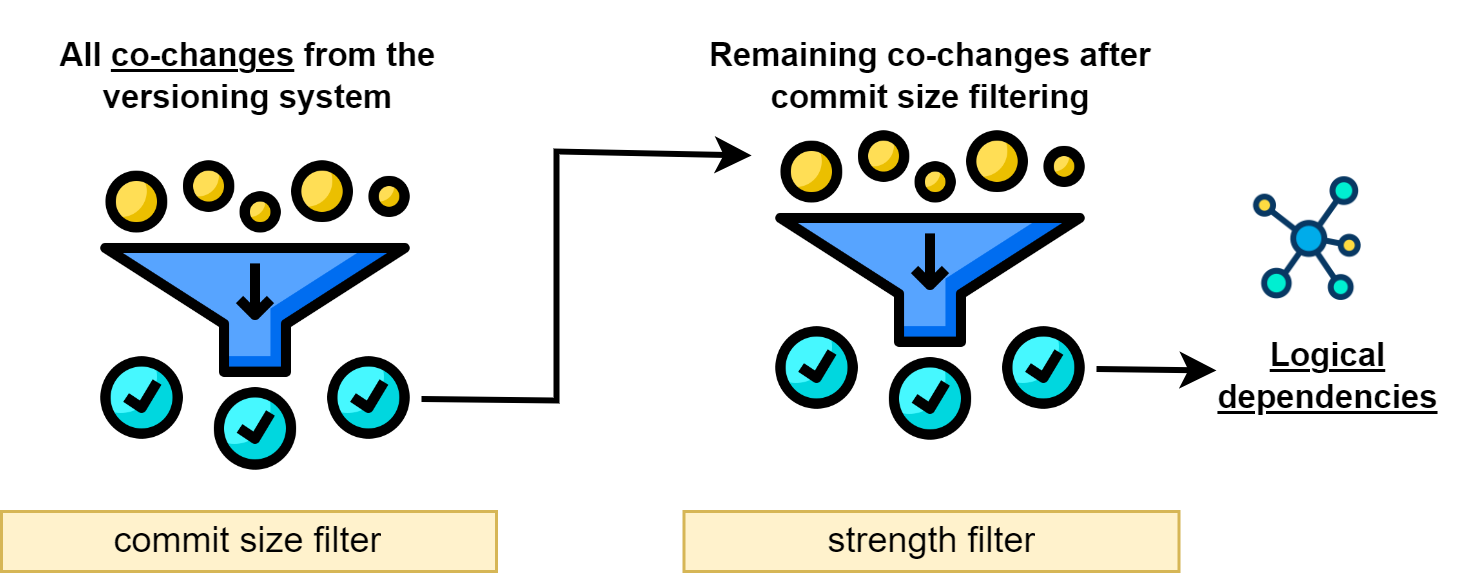
\includegraphics[width=\columnwidth]{filtering.png}
  \caption{Filter application process}
  \label{fig:filtering}
\end{figure}

\subsubsection{Dependency Extraction and Filtering Tool}

To extract and filter the co-changes, we used a previously developed tool \cite{b4}. This tool takes the GitHub repository address and the threshold values for commit and strength filters as input. The tool clones the repository, downloads all commit diffs starting from the first commit, examines all files changed in each commit to identify which entities have changed in those files, and creates undirected co-change dependencies between all changed entities within a commit.

The commit size filter is applied to these undirected co-change dependencies since the metric value for $(A \rightarrow B)$ is the same as for $(B \rightarrow A)$. For the strength filter, each co-change dependency is converted into a directed co-change dependency, so for each $(A \rightarrow B)$ dependency, we have both $(A \rightarrow B)$ and $(B \rightarrow A)$. This conversion is necessary because, as mentioned in the previous section, the confidence filter evaluates the rule's antecedent. Thus, the metric value for $(A \rightarrow B)$ differs from the metric value for $(B \rightarrow A)$.

After applying the filters, the remaining dependencies are exported to a CSV file for further use.

It is important to note that the strength metric is only used for filtering and is \textit{not considered as a weight} of the dependencies. The \textit{weight assigned to each dependency is the number of commits in which both entities were updated together}.


\section{Combining Structural and Logical Dependencies}


\begin{figure}[t!]
  \centering
  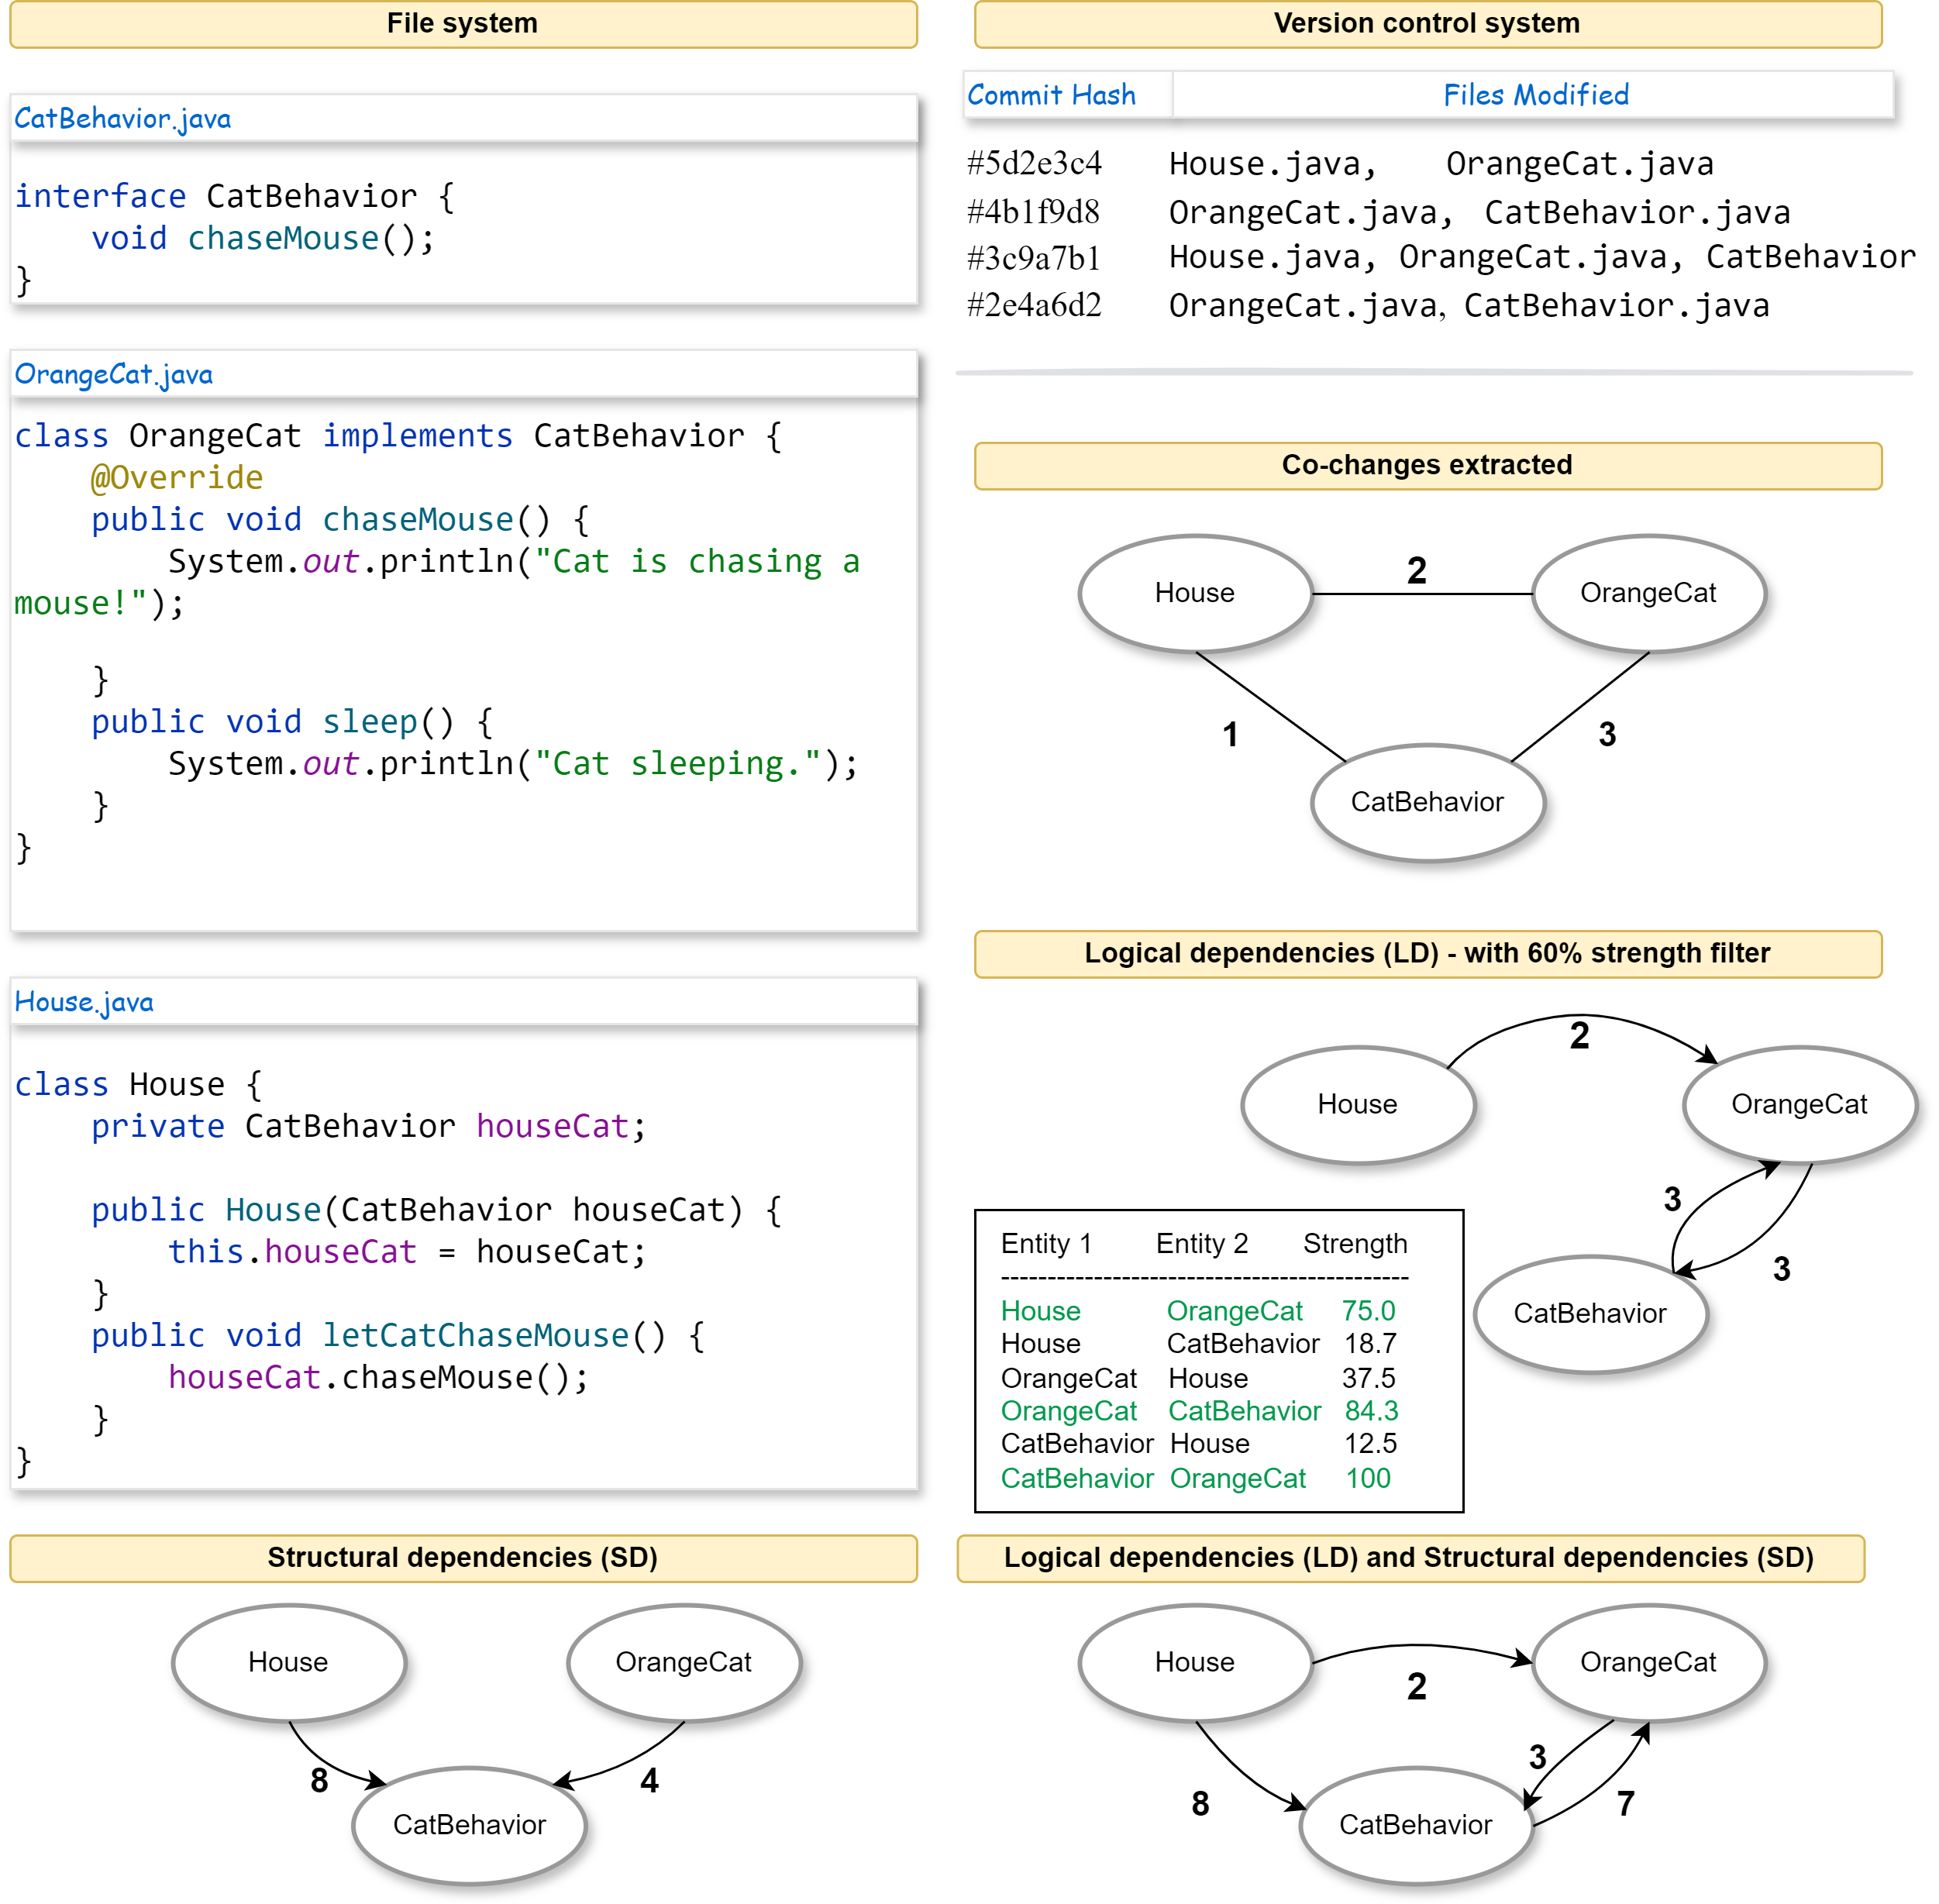
\includegraphics[width=\columnwidth]{codegraph.png}
  \caption{Dependency Graph: Combining structural and logical dependencies.}
  \label{fig:codegraph}
\end{figure}

When structural dependencies (SD) and logical dependencies (LD) are combined in software clustering, both types of relationships are represented within the same graph.

Each entity in the system is represented as a node in the graph, and the dependencies between them are represented as directed weighted edges.

\textit{SD and LD weights are combined} when the same pair of entities appear in both dependencies. In this case, the weights from SD and LD are summed, giving more influence to those entity pairs. When a pair of entities appear only in SD or only in LD, the edge is added to the graph together with its corresponding weight.

Figure \ref{fig:codegraph} illustrates combining structural and logical dependencies in the same dependency graph. The structural dependencies between \texttt{House}, \texttt{OrangeCat}, and \texttt{CatBehavior} entities are visible from the source code analysis.

However, the combination of SD and LD reveals additional insights. One important observation is the logical dependency between \texttt{House} and \texttt{OrangeCat}, which is not observed from the structural analysis. This relation is extracted from version control and filtered using a 60\% strength filter. The strength metric reveals that \texttt{House} and \texttt{OrangeCat} have a significant co-change value of 75.0, usually associated with a strong relationship.

When SD and LD overlap, such as between \texttt{OrangeCat} and \texttt{CatBehavior}, their weights are summed. This summation increases the weight of the dependency, making it more important in the dependency graph.




New structure:
\begin{verbatim}
Chapter 3: Research methodology
    3.1 Overview of research approach
    3.2 Data collection
        3.2.1 Extracting structural dependencies
        3.2.2 Extracting logical dependencies (co-changing pairs)
        3.2.3 Description of data sets used
    3.3 Tool development
        3.3.1 Tool for measuring software dependencies
    3.4 Filtering logical dependencies
        3.4.1 Filtering based on commit transaction size
        3.4.2 Filtering based on number of occurrences
        3.4.3 Filtering based on connection strength

Chapter 4: Combining structural and logical dependencies
    4.1 Analysis of dependency overlaps
        4.1.1 Measurements of overlaps
        4.1.2 Implications of overlaps
    4.2 Weight assignment
        4.2.1 Structural dependencies weights
        4.2.2 Logical dependencies weights
    4.3 Integration techniques
        4.3.1 Methods for combining dependencies
        4.3.2 Combination framework
\end{verbatim}